\documentclass[tikz,border=4pt]{standalone}
\begin{document}
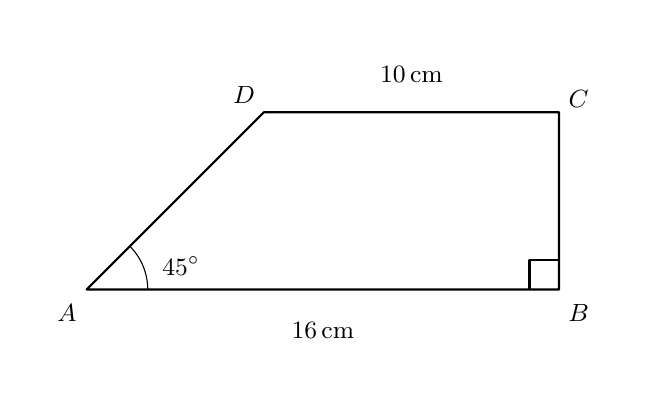
\begin{tikzpicture}[x=0.025cm,y=-0.025cm]
\path[use as bounding box] (0,0) rectangle (300,175);
\draw[black,line width=0.8pt,line join=round] (30,133) -- (270,133) -- (270,43) -- (120,43) -- cycle;
\draw[black,line width=0.8pt,line join=round] (255,133) -- (255,118) -- (270,118);
\draw[black,line width=0.4pt,line join=round] (51.9203,111.0797) -- (52.6258,111.8086) -- (53.307,112.5603) -- (53.9633,113.3338) -- (54.594,114.1284) -- (55.1982,114.9432) -- (55.7756,115.7773) -- (56.3253,116.6299) -- (56.8468,117.5) -- (57.3396,118.3867) -- (57.8031,119.2891) -- (58.2368,120.2061) -- (58.6403,121.1368) -- (59.0131,122.0802) -- (59.3548,123.0354) -- (59.6652,124.0012) -- (59.9437,124.9766) -- (60.1902,125.9606) -- (60.4043,126.9522) -- (60.5859,127.9502) -- (60.7348,128.9537) -- (60.8507,129.9615) -- (60.9336,130.9725) -- (60.9834,131.9857) -- (61,133);
\node[font=\small,inner sep=0pt] at (78,121) {$45^\circ$};
\node[font=\small,inner sep=0pt] at (20,145) {$A$};
\node[font=\small,inner sep=0pt] at (280,145) {$B$};
\node[font=\small,inner sep=0pt] at (280,36) {$C$};
\node[font=\small,inner sep=0pt] at (110,34) {$D$};
\node[font=\small,inner sep=0pt] at (150,154) {$16\,\mathrm{cm}$};
\node[font=\small,inner sep=0pt] at (195,24) {$10\,\mathrm{cm}$};
\end{tikzpicture}
\end{document}
